\subsection{Simulação 1}

A simulação 1 consiste em um Reator de Batelada, no qual estão dispostas 3 materiais que serão jogados para fabricação de um produto.

Primeiramente foi descrito as entradas e saídas do sistema por meio das tabelas \ref{tbl:1} e \ref{tbl:2}. 

\begin{longtable}[]{@{}lcc@{}}
\toprule
Entradas & Nv. comportamental & Nv. tecnológico \\
\midrule
\endhead
Chave de nível superior & \(S_H\) & S\_H \\
Chave de nível inferior & \(S_L\) & S\_L \\
\bottomrule
\caption{Descrição das entradas para a simulação 1.}
\label{tbl:1}
\end{longtable}

\begin{longtable}[]{@{}lcc@{}}
\toprule
Saídas & Nv. comportamental & Nv. tecnológico \\
\midrule
\endhead
Válvula do material A & \(V_A\) & V\_A \\
Válvula do material B & \(V_B\) & V\_B \\
Válvula do material C & \(V_C\) & V\_C \\
Válvula de segurança & \(V_S\) & V\_S \\
Válvula de descarga & \(V_D\) & V\_D \\
Bomba & \(B\) & B \\
Agitador & \(A\) & A \\
\bottomrule
\label{tbl:2}
\end{longtable}

Acerca dos níveis assumidos por cada variável, as chaves de nível $S_L$ e $S_H$ assumirão nível lógico alto quando estas identificarem que aquele nível foi alcançado. No caso do reservatório estar completamente vazio, significa que ambas as chaves de nível estarão em nível lógico baixo. Em relação às demais saídas, para as válvulas o nível lógico alto significa que estarão abertas e para a bomba e agitador, significam que estão em funcionamento.

Por meio da figura \ref{sim1} que ilustra o processo descrito na linguagem SFC, pode-se tirar as seguintes conclusões acerca do funcionamento das etapas.

\begin{itemize}
    \item Etapa 0 (E0):
    
    A etapa E0 configura-se como a etapa inicial. Ela marca o início do processo quando o reservatório está vazio e só poderá transitar para a etapa E1, E2 e E3 quando estiver certo de que ambas as chaves $S_H$ e $S_L$ estão em nível lógico baixo.
    
    \item Etapa 1, 2 e 3 (E1, E2 e E3):
    
    As etapas E1, E2 e E3 ocorrem concorrentemente, indicadas pelo paralelismo no diagrama SFC. Ao identificar o nível baixo, cada uma das etapas anteriores executarão suas ações associadas, permitindo assim que as três válvulas $V_A$, $V_B$ e $V_C$ sejam acionadas simultaneamente, permitindo que o reservatório seja preenchido.
    
    O preenchimento total será indicado quando ambas as chaves de nível $S_H$ e $S_L$ estiverem em nível lógico alto, permitindo assim transitar para a etapa 4 (E4).
    
    \item Etapa 4 (E4):
    
    A etapa E4 garante que a chave de nível alto $S_H$ não permaneça ligada. Para isso ele ativa a válvula de segurança $V_S$ para que o nível do reservatório reduza um pouco, evitando que uma possível falha nas válvulas que despejam materiais prejudique o processo.
    
    A transição da etapa E4 para a etapa E5 se dá quando a chave de nível alto $S_H$ não mais está em nível lógico alto.
    
    \item Etapa 5 (E5):
    
    Logo quando a etapa E5 é alcançada o agitador é ligado por 10 segundos por meio de uma ação limitada em tempo. Concorrente a isso existem duas outras ações com retardo de 10 segundos, que permitirão acionar a válvula de descarga e o motor para impulsionar a descarga. 
    
    A transição da etapa E5 para a etapa inicial E0 só é realiza quando a chave de nível baixo $S_L$ assume o nível lógico baixo, indicando que o reservatório está vazio, permitindo reiniciar o processo.
\end{itemize}


\begin{figure}[H] 
\centering
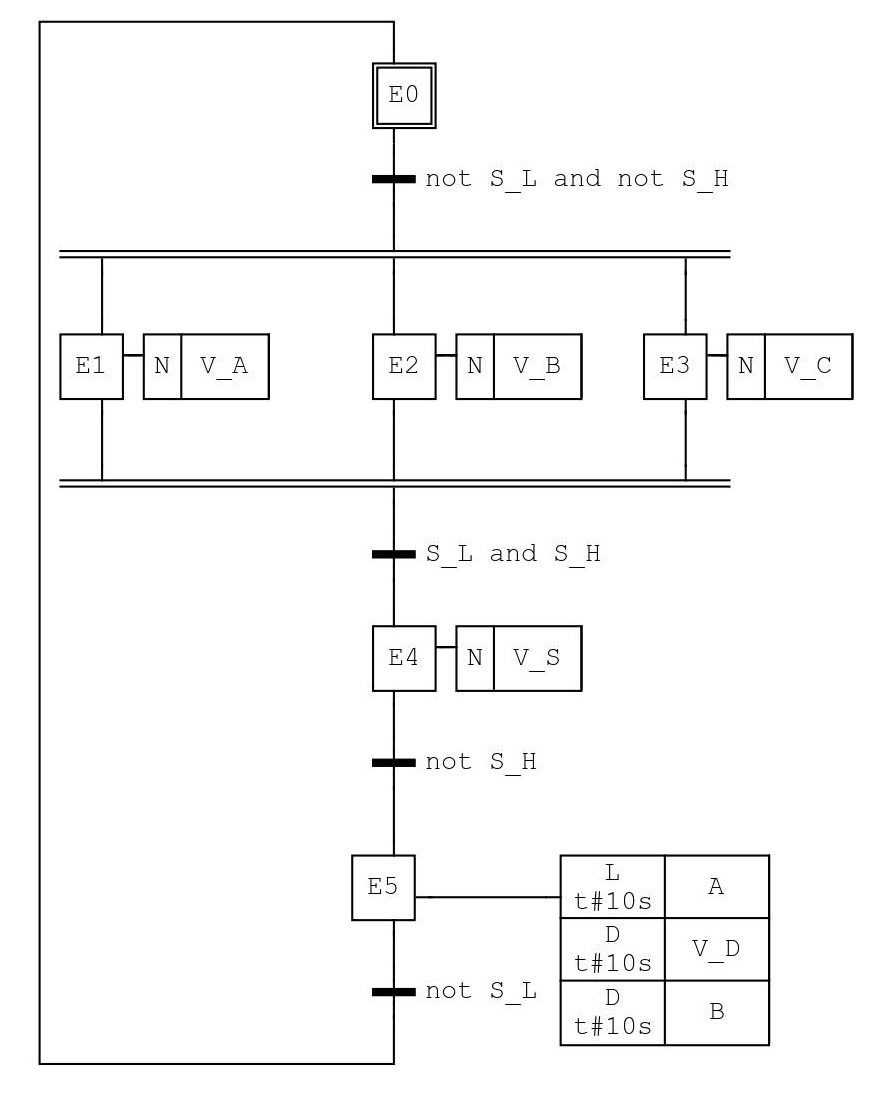
\includegraphics[width=9cm]{images/sim1.jpg}
\caption{Diagrama em SFC para a primeira simulação.}
\label{sim1} 
\end{figure}